\documentclass[a4paper]{article}
\usepackage{algorithmicx}
\usepackage{float}
\usepackage{algpseudocode}
\usepackage{graphicx}
\usepackage{vmargin}
\usepackage[utf8]{inputenc}
\usepackage{mdwlist}
\setpapersize{A4}
\setmargins{2.5cm}       % margen izquierdo
{1.5cm}                        % margen superior
{16.5cm}                      % anchura del texto
{23.42cm}                    % altura del texto
{10pt}                           % altura de los encabezados
{1cm}                           % espacio entre el texto y los encabezados
{0pt}                             % altura del pie de página
{2cm}                           % espacio entre el texto y el pie de página
\makeatletter
\setlength{\@fptop}{0pt}
\makeatother
\begin{document}
\section*{Metaheurística GRASP}
\subsection*{a) Explicación del algoritmo}
El algoritmo básicamente itera una cantidad de veces, en principio desconocida, y aplica primero la heurística golosa aleatorizada (con distintos valores de alfa). Una vez que tiene una solución factible generada por la heurística golosa aleatorizada, aplica un algoritmo heurístico de busqueda local sobre ella, obteniendo una solución nueva, mejor o igual (nunca peor). Como hay dos algoritmos distintos de búsqueda local (utilizan distintas vecindades), GRASP siempre va a elegir el mismo durante una ejecución y va a estar determinado por un parámetro de entrada.
\newline Otra cosa configurable en GRASP es quienes van a formar parte de la RCL. Considerando lo que explicamos sobre el algoritmo goloso y sus distintas decisiones y criterios, en realidad existen tres listas restrictas de candidatos:
\begin{itemize}
\item La que está conformada por los pares de nodos candidatos a ser la arista "máxima" que tome el algoritmo en la etapa inicial.
\item La que dado un nodo $u$ está conformada por los posibles pares de $u$ (ver definición de Par en la explicación de la heurística golosa).
\item La que a la hora de ubicar un nodo o un par de nodos dentro de la partición $P$, contiene los pares de posiciones que son candidatos a "la mejor manera" de ubicar los nodos.
\end{itemize} 

\vspace{0.4cm}
\noindent Estas listas de candidatos son construidas en base a tres parámetros, uno para cada una, $alfa$, $beta$, $gamma$. Cada uno de esos parámetros representa un porcentaje, que indica que tan distantes pueden estar del valor óptimo los valores contenidos en cada lista.
\newline \newline La cantidad de veces que itera el algoritmo va a estar relacionado con la cantidad de mejoras que hubo en las últimas iteraciones. Se trata de un valor entero configurable (otro parámetro, aca vamos a llamarlo $delta$), de manera tal que representa una cantidad de iteraciones. Si se hizo esa cantidad de iteraciones de manera seguida y no se observó ninguna mejora en la solución con la que se está trabajando, entonces el algoritmo termina.
\newline La solución devuelta por GRASP siempre es la mejor encontrada hasta el momento, esto significa que se va almacenando y se pisa cuando se encuentra una solución mejor.
\vspace{0.5cm}
\subsection*{a) Experimentación}
Las instancias que generamos para realizar la experimentación de la calidad de las soluciones y la performance de GRASP, fueron grafos completos. Al igual que como experimentamos con otros algoritmos, los pesos de las aristas de los grafos completos se determinaron de manera aleatoria en un rango de 0 a 50.
\newline Todas las mediciones que presentaremos a continuación se realizaron sobre el mismo conjunto de instancias, el cual tiene 100 grafos completos con vértices de 1 a 100.
\newline El objetivo de esta experimentación es poder encontrar una configuración conveniente de los parámetros de GRASP y ver si se adapta a otros grafos que no necesariamente sean completos.
\newline
\newline Vamos a presentar gráficos comparativos sobre la performance y la calidad de las soluciones que nos brinda GRASP con distintas configuraciones.
Cuando hablemos de Vecindad 1 y Vecindad 2, vamos a estar haciendo referencia al primer y segundo algoritmo de búsqueda local que presentamos.
\begin{figure}[H]
\centering
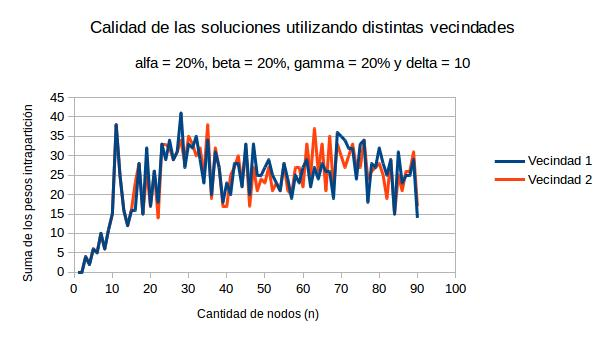
\includegraphics[scale=0.7]{20202010.jpg}\caption{En este experimento los porcentajes que determinan las RCL se mantienen bajos. También, delta es un número relativamente bajo. Podemos observar que el algoritmo con esa configuración, utilizando la vecindad 1, brinda soluciones de peso mayor en casi todos los casos, que cuando utiliza la vecindad 2. Por lo cual, en calidad de soluciones podemos decir que conviene utilizar la vecindad 2.}
\end{figure}

\begin{figure}[H]
\centering
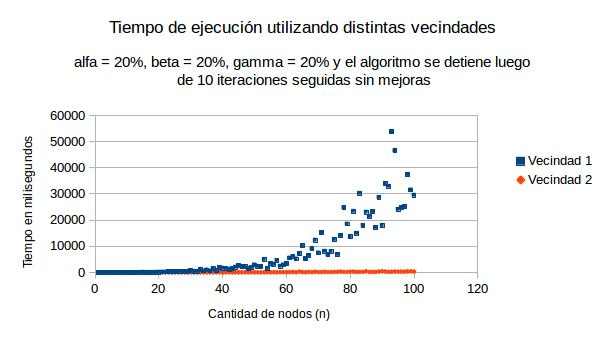
\includegraphics[scale=0.7]{20202010c.jpg}\caption{En este gráfico, podemos contemplar la enorme diferencia entre el tiempo de ejecución de GRASP utilizando una vecindad y la otra. Es importante ver que GRASP utilizando la vecindad 2 es mucho más rápido y casualmente era con la vecindad 2 (con esta misma configuración y con este conjunto de instancias) que GRASP nos daba soluciones mejores. Claramente con estos valores de alfa, beta, gamma y delta, el algoritmo funciona mejor utilizando la vecindad 2.}
\end{figure}

\begin{figure}[H]
\centering
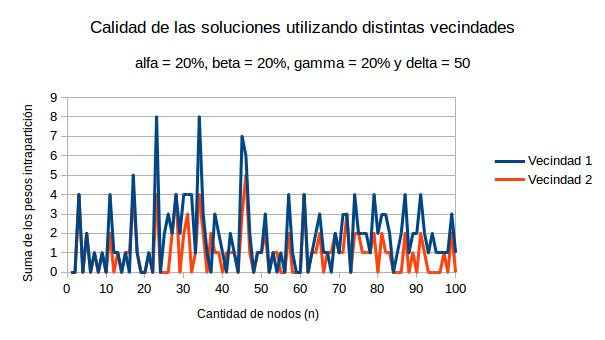
\includegraphics[scale=0.7]{20202050.jpg}\caption{
\noindent En este caso decidimos aumentar delta. Intuitivamente podríamos creer que el hecho de aumentar esto nos puede llegar a dar soluciones mejores, debido a que aumentan las chances de encontrar una mejor solución. En este caso esto efectivamente se cumplió en algunas instancias.}
\end{figure}

\begin{figure}[H]
\centering
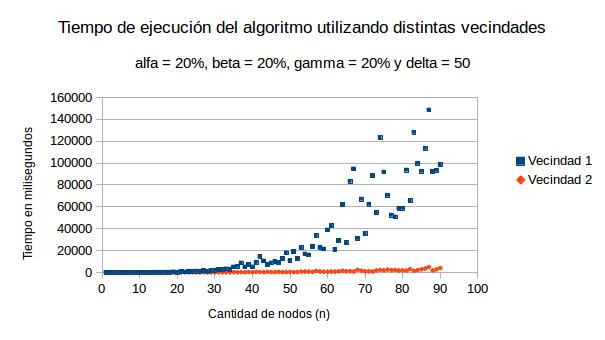
\includegraphics[scale=0.7]{20202050c.jpg}\caption{Podemos observar también como el tiempo de ejecución del algoritmo al aumentar ese parámetro, se incrementa bastante. De todas formas, como decidimos que la mejor vecindad para este caso es la 2, vamos a ver que tanto empeora el tiempo de ejecución y que tanto mejoran las soluciones en relación a los datos anteriores, pero utilizando solo la vecindad 2. Será en los siguientes gráficos que mostraremos esto.}
\end{figure}

\begin{figure}[H]
\centering
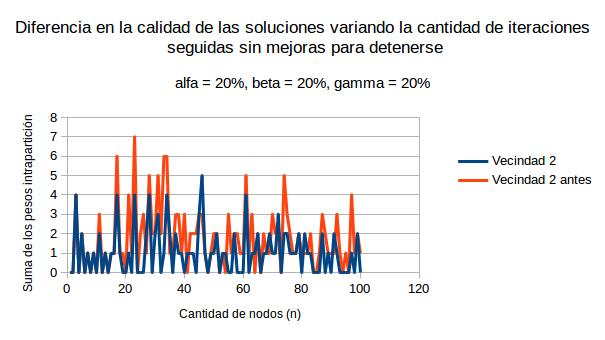
\includegraphics[scale=0.7]{20202020difcal.jpg}\caption{Vemos como efectivamente si aumentamos delta obtenemos soluciones mejores.}
\end{figure}

\begin{figure}[H]
\centering
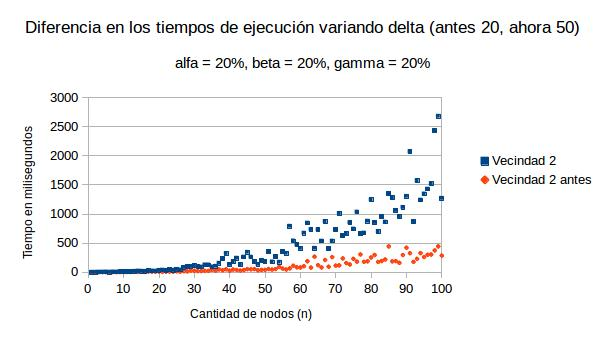
\includegraphics[scale=0.7]{202020difcom.jpg}\caption{En el gráfico anterior pudimos ver "lo que ganamos" al aumentar el delta. En este gráfico podemos ver lo que nos cuesta aumentar el delta. Es claro ver que el tiempo de ejecución va aumentar si el delta aumenta. De todas formas, en este caso el aumento no es demasiado grande y algunas soluciones son significativamente mejores, con lo cual parece razonable aumentar el tiempo de ejecución con el objetivo de mejorar nuestras soluciones.}
\end{figure}

\begin{figure}[H]
\centering
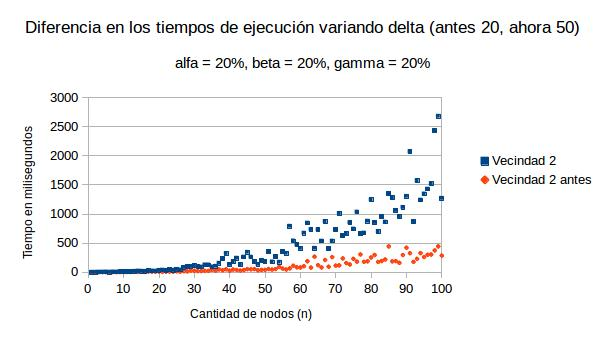
\includegraphics[scale=0.7]{202020difcom.jpg}\caption{En el gráfico anterior pudimos ver "lo que ganamos" al aumentar el delta. En este gráfico podemos ver lo que nos cuesta aumentar el delta. Es claro ver que el tiempo de ejecución va aumentar si el delta aumenta. De todas formas, en este caso el aumento no es demasiado grande y algunas soluciones son significativamente mejores, con lo cual parece razonable aumentar el tiempo de ejecución con el objetivo de mejorar nuestras soluciones.}
\end{figure}

\begin{figure}[H]
\centering
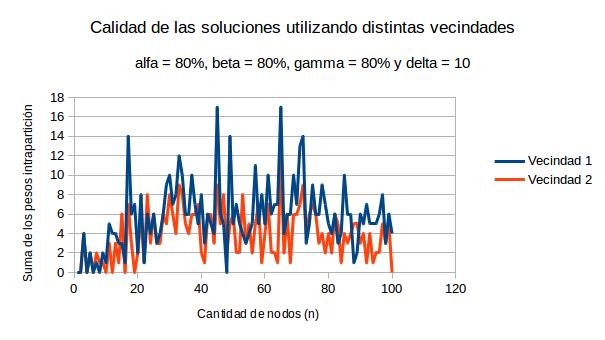
\includegraphics[scale=0.7]{80808010.jpg}\caption{Ahora, probamos aumentar bastante los parámetros alfa, beta y gamma. Lo que produce esto es aumentar el tamaño de nuestras listas de candidatos (ya que ahora podrán estar dentro de ellas los que cumplan estar hasta un 80\% lejos del mejor). Vemos que las soluciones que provee GRASP utilizando la vecindad 2 siguen siendo mejores que las que provee cuando utiliza la 1. Empezamos a pensar que esto es independiente de los parámetros alfa, beta, gamma y delta.}
\end{figure}

\begin{figure}[H]
\centering
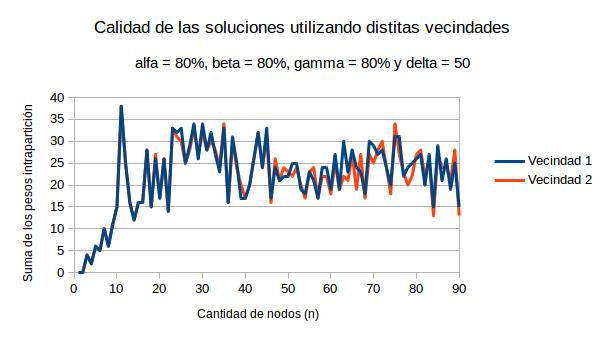
\includegraphics[scale=0.7]{80808050.jpg}\caption{Una vez más, aumentamos el delta y vemos que, con ambas vecindades, obtenemos soluciones mejores. Sin embargo, la vecindad 2 sigue predominando sobre la 1 en calidad de soluciones.}
\end{figure}
\noindent Dado que las soluciones que provee GRASP con la vecindad 2 siempre son mejores a las que provee cuando hace uso de la vecindad 1 y, además, es significativamente más lento cuando usa esta última (lo vimos en el gráfico 4 y además la complejidad teórica del algoritmo que usa esa vecindad es mayor a que usa la vecindad 2), claramente conviene correr GRASP con la vecindad 2. Por otra parte, vimos también que si aumentamos el parámetro delta, si bien el tiempo de ejecución aumenta, también mejoran las soluciones que obtenemos. Una buena configuración entonces, estaría determinada por delta $\sim 50$ y la vecindad 2. Restaría ver qué parámetros de alfa, beta y gamma nos conviene utilizar.

\begin{figure}[H]
\centering 
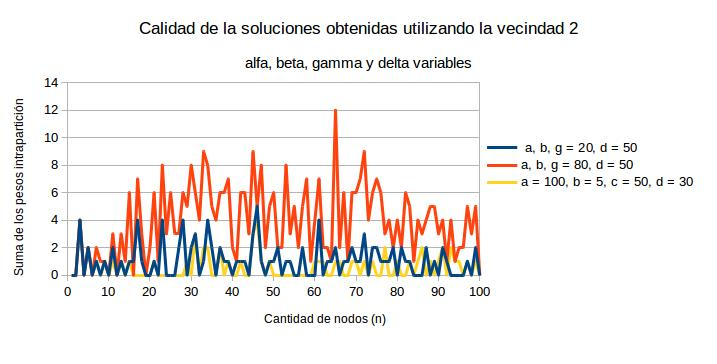
\includegraphics[scale=0.7]{vecindad2variaabgd.jpg}
\end{figure}

En el gráfico de arriba, podemos observar la calidad de las soluciones obtenidas con tres configuraciones distintas de alfa, beta y gamma. Entre estas tres configuraciones distintas, se encuentran dos de las que mencionamos arriba y una nueva en la cual a, b y g no tienen los mismos valores y el valor de delta es 30. Esta nueva configuración fue elegida para poder ver si el hecho de variar los tamaños de las RCL's puede llegar a aumentar las chances de obtener mejores soluciones.
\newline En el gráfico podemos ver que la nueva configuración que varía los tamaños de las RCL's es la que mejores soluciones nos da. Si bien en algunos casos la combinación alfa = beta = gamma = 20 y delta = 50 da mejores soluciones, en la mayoría de los casos la nueva configuración le gana.
\newline Podemos concluir entonces que una buena configuración para estos casos, es variar el alfa, beta y gamma de manera que las RCL's tengan distinto tamaño y que el delta sea "mediano". De esta forma, un valor "mediano" de delta no nos recorta demasiadas soluciones, pero tampoco incrementa demasiado el tiempo de ejecución.
\end{document}